\section{Architectural Evolution}
\label{sec:architectural_evolution}

The final \texttt{G3} revision of the \texttt{DetectorNX} architecture was not the result of a single design phase,
but rather the culmination of an iterative engineering process across four distinct generations.
According to the project's success criteria, the model required both high temporal precision and robust spatial localization.
This section documents the empirical obstacles encountered during development, and the actionable insights that led to the final optimized configuration.

\subsection{Phase 0: The Spatial Cropping Pitfall (Early Prototyping)}

Prior to the implementation of downsampling in the \gls{bolt} pipeline, early prototyping explored the use of aggressive spatial cropping to bypass the computational costs of high-definition event processing.

\subsubsection{Architectural Intent \& Technical Logic}
The primary objective of this phase was to establish a high-resolution localized baseline by cropping the raw $1280 \times 720$ \gls{etram} sensor data into a $224 \times 224$ patch,
as illustrated in Figure \ref{fig:preprocessing_pipeline}; these patches were deterministically anchored to the centroid of the ground-truth vehicle annotation. 

The technical logic was based on improving the \gls{snr} at the network's input;
through \textit{localised foveation}, the initial stem layers would receive a significantly higher frequency of spikes per pixel on the target object. 
This denser spike signal would preserve fine geometric detail often attenuated by global downsampling, while the smaller patches avoided the memory overhead of aggressive pooling.

\subsubsection{Empirical Obstacle: Constant Target Bias}
During initial training cycles, the model achieved exceptional accuracy metrics. 
However, because the pipeline used deterministic centroid-anchored cropping, the target vehicle occupied the geometric centre of every training sample, and the \gls{snn} succumbed to \textit{Constant Target Bias}: a severe form of spatial overfitting where the regression head ignores the visual event stream and learns to output a constant coordinate vector.

Critically, this collapse was invisible to the \gls{iou} metric, since the validation split inherited the same cropping as training. 
The bias only surfaced when inference was later run on raw full-frame input, where the predicted box consistently sat near the image centre regardless of the vehicle's true position (Figure~\ref{fig:constant_target_bias}).

\begin{figure}[h]
    \centering
    \begin{subfigure}[b]{0.32\textwidth}
        \centering
        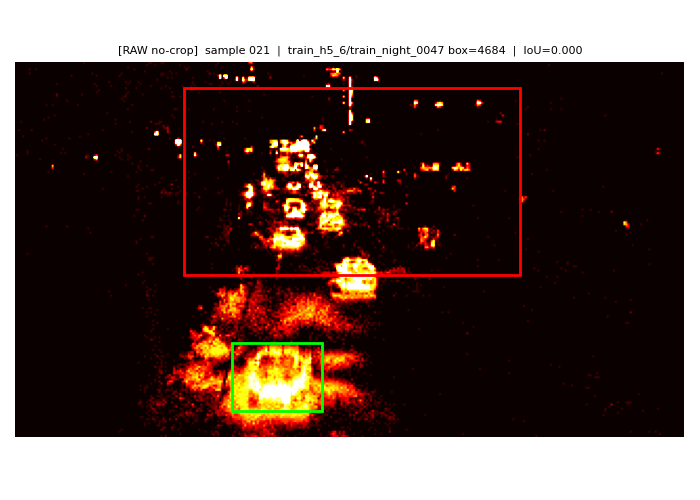
\includegraphics[trim=15 63 16 62, clip, width=\textwidth]{chapter_3/dnx_results/constant_target_bias/sample_021.png}
        \caption{Train sample, \gls{iou}$=0.000$.}
        \label{fig:ctb_a}
    \end{subfigure}
    \hfill
    \begin{subfigure}[b]{0.32\textwidth}
        \centering
        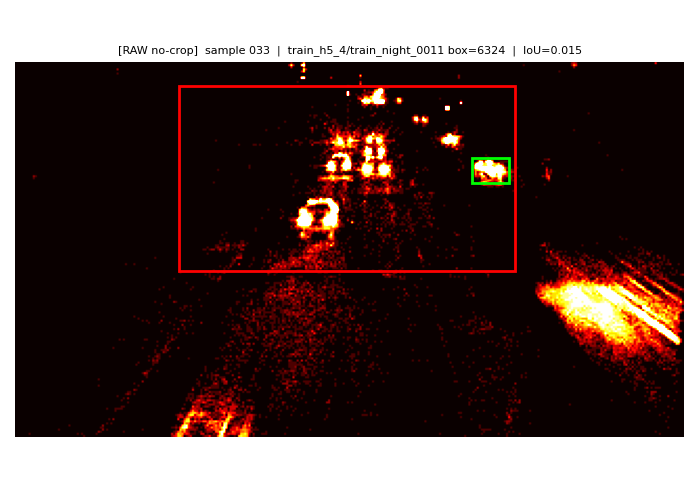
\includegraphics[trim=15 63 16 62, clip, width=\textwidth]{chapter_3/dnx_results/constant_target_bias/sample_033.png}
        \caption{Train sample, \gls{iou}$=0.015$.}
        \label{fig:ctb_b}
    \end{subfigure}
    \hfill
    \begin{subfigure}[b]{0.32\textwidth}
        \centering
        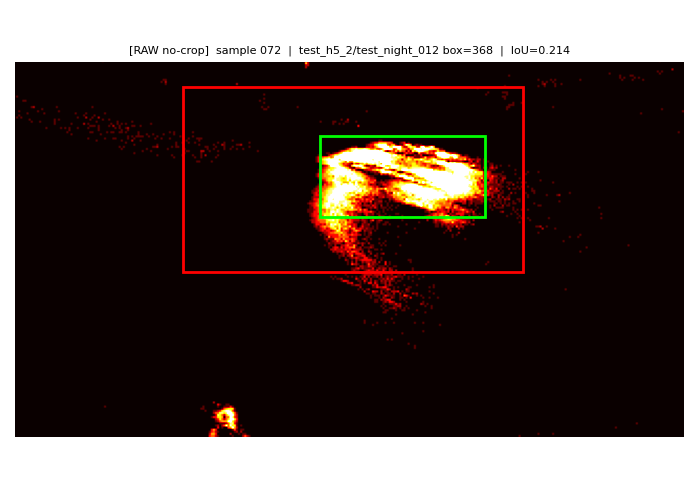
\includegraphics[trim=15 63 16 62, clip, width=\textwidth]{chapter_3/dnx_results/constant_target_bias/sample_072.png}
        \caption{Test sample, \gls{iou}$=0.214$.}
        \label{fig:ctb_c}
    \end{subfigure}
    \caption[Constant Target Bias failure mode]{Qualitative evidence of \textit{Constant Target Bias} during Phase 0. Across three raw full-frame samples drawn from the training and test splits, the \gls{snn} regression head (red) emits a near-identical large central bounding box while the ground-truth vehicle (green) varies in position and scale between scenes. The marginally higher overlap in (\subref{fig:ctb_c}) arises only because the target vehicle incidentally sits near the image centre where the predicted box anchors, confirming the model has learned a constant coordinate shortcut rather than extracting vehicle features from the event stream.}
    \label{fig:constant_target_bias}
\end{figure}

\subsubsection{Actionable Insight}
This phase provided a critical methodological lesson: for a spiking architecture to learn robust spatial localization and objectness, it must be exposed to targets moving dynamically relative to the sensor boundaries within a full-frame (or semi-full-frame) field of view. This insight led to the total abandonment of centered cropping in favor of the global $4\times$ spatial downsampling strategy utilized in the final \gls{bolt} pipeline, ensuring that the model learned to correlate visual spike patterns with absolute spatial coordinates.

\subsection{Generation 1 (G1): The Multi-Box Paradigm Shift}

Following the resolution of the spatial cropping bias, the architecture progressed to full-frame processing. 
However, this transition immediately exposed fundamental limitations in the network's predictive capabilities regarding multi-object scenes.

\subsubsection{Architectural Intent \& Technical Logic}
The primary objective of this phase was to develop a \textit{scene-aware detector} capable of identifying multiple vehicles simultaneously within the \gls{etram} traffic environment. 
To achieve this, the network's output topology underwent a paradigm shift, transitioning from a simplistic single-box regression head (which output a single $[x, y, w, h]$ vector) to a Multi-Box Regression Head with a fixed-capacity output of $[B, 5, 5]$, where there are 5 features $(x, y, w, h, mask)$ and 5 bounding boxes predicted per inference.
The technical logic dictated that the network required a mechanism to independently evaluate distinct spatial regions. 
To facilitate this, each of the five predicted boxes was augmented with a fifth dimension: an ``Objectness'' or Confidence Score. 
This structural addition allowed the model to not only regress bounding box coordinates but also to gate its own predictions, learning to suppress background artifacts with low confidence while maintaining high confidence for legitimate structural targets.

\subsubsection{Empirical Obstacle: Single-Target Ambiguity \& Label Noise}
Initial prototypes with the standard single-box head proved fundamentally incompatible with multi-vehicle scenes: the backbone naturally extracted features for all visible vehicles, but the single-target label penalised correct detections of secondary vehicles as errors, introducing severe label noise. 
Over thousands of iterations, the model minimised this ambiguous loss by averaging positions across visible vehicles, producing predictions that hovered meaninglessly between cars or a ``super-box'' encompassing the entire roadway.

\todo[inline,backgroundcolor=myblue,textcolor=white]{Insert images of the super box.}

\subsubsection{Actionable Insight: The Vectorized Matching Loss}
This phase highlighted the need for a mechanism to handle the \textit{Assignment Problem}: determining which of the 5 predicted boxes should be compared against which ground-truth vehicle. 
The resulting Vectorized Multi-Box Loss computes a 3D matrix of \gls{iou} overlaps between the 5 predictions and the $M$ ground-truth objects per batch, then uses greedy matching to identify the best match per real vehicle. 
Only matched boxes receive a \textit{coordinate gradient}; all unmatched boxes are assigned a target confidence of $0.0$, penalising false positives and suppressing the Ghost Detections prevalent in earlier iterations.

The actionable insight was the development of a Vectorized Multi-Box Loss. This computational innovation calculates a 3D matrix of all possible \gls{iou} overlaps between the 5 predictions and the $M$ ground truth objects in every batch. Utilizing greedy matching, the loss function identifies the best match for each real vehicle in the scene. Only this matched predicted box receives a \textit{coordinate gradient}, signaling it to move closer to the target. 

Crucially, all unmatched predicted boxes are assigned a target confidence of $0.0$, acting as a metabolic penalty for false positives. This forces the model to learn that predicting a vehicle where none exists carries a heavy mathematical penalty, effectively cleaning up the \gls{snn}'s vision and reducing the Ghost Detections prevalent in early iterations. 

The transition from single-box regression to scene-aware multi-box detection also introduced the Multi Box Label Alignment step of the \gls{bolt} pipeline (Figure~\ref{fig:preprocessing_pipeline}). 
By resolving the spatial ambiguity of multi-vehicle traffic, the new head transformed contradictory Label Noise into a structured multi-target learning signal, which was essential for stable convergence on the high-definition, high-density event streams of the \gls{etram} dataset.

\subsection{Generation 2 (G2): The Expanded Spatial Head (7.00M Parameters)}

While Generation 1 successfully established the multi-box logic, empirical validation revealed a persistent failure mode characterized by ghost Detections and overlapping predictions.

\subsubsection{Architectural Intent \& Empirical Obstacle}
The primary objective of this phase was to resolve \textit{Information Congestion} within the regression head. 
Generation 1 architecture utilized an Adaptive Average Pooling layer of $4 \times 4$, compressing the entire field of view into just 16 spatial blocks before entering the final linear layers.

This severe spatial bottleneck meant that when vehicles were in close proximity, or situated near clusters of sensor artifacts, their respective spiking features were averaged into an identical $4 \times 4$ block. 
The regression head lacked the spatial memory required to distinguish valid target spikes from background noise. 
Consequently, the model frequently outputted overlapping bounding boxes for a single vehicle or failed to suppress high-confidence noise, resulting in an inflated average of 2.50 detections per frame - significantly higher than the ground truth average of 2.02.

\subsubsection{Actionable Insight: Quadrupling Spatial Memory}
To resolve this congestion, the Adaptive Pooling resolution was expanded from $4 \times 4$ to $8 \times 8$, 
quadrupling the spatial memory to 64 distinct blocks and providing the regression head with a finer structural map of backbone activations. 
This enabled localized Object-Noise Discrimination: the model could now isolate structured vehicle spike trains from surrounding sensor noise, producing significant Confidence Polarization with real-object scores surging to $0.99$ while background noise was pushed toward $0.0$.

Average detections per frame (ADP) dropped to 2.06, closely matching the ground truth of $2.02$. However, the Mean \gls{iou} plateaued at 41\%, confirming the backbone's heavy downsampling remained the fundamental bottleneck for geometric precision.

\subsection{Generation 3 (G3): The High-Resolution Backbone (11.7M Parameters)}

Following the expansion of the spatial head in Generation 2, the model demonstrated excellent selectivity but remained computationally constrained by its geometric precision.

\subsubsection{Architectural Intent \& Empirical Obstacle}
The primary objective of this final phase was to break the Precision Ceiling established in Generation 2.

The fundamental obstacle was the severe spatial compression occurring within the backbone. By the final layer, the feature map had been downsampled to an $11 \times 20$ resolution. 
At this scale, a single pixel in the final feature map represented a massive $16 \times 16$ area of the original HD sensor. 
Consequently, if a vehicle's bounding box edge shifted by several pixels in the real world, the network was entirely blind to the change; the G2 generation simply lacked the geometric detail required to draw tight, pixel-perfect bounding boxes.

Furthermore, an analysis of the network's information flow revealed that the Generation 2 backbone was suffering from neural silencing, exhibiting an average firing rate of $< 1.5\%$. This extreme sparsity starved the regression head of the necessary temporal evidence required for high-confidence predictions.

\subsubsection{Actionable Insight: Semantic Expansion \& Metabolic Awakening}
To overcome this precision ceiling, a multi-faceted architectural overhaul was implemented to create the final G3 configuration:

\begin{itemize}
    \item \textbf{Resolution Boost \& Semantic Depth:} To provide the necessary geometric detail, the convolution stride in Block 3 was reduced to $s=1$. This effectively halted the downsampling earlier in the network, doubling the final feature map resolution to $22 \times 40$ (quadrupling the available spatial cells to 880). To handle the increased complexity and high-frequency sensor artifacts exposed by this higher resolution, the backbone's semantic was expanded via the addition of a 4th \texttt{SEWResBlock} (512 channels). 
    This allowed the network to think deeper about the structural composition of the vehicle.
    
    \item \textbf{Metabolic Regularization:} 
    The \gls{lif} firing threshold was lowered ($V_{th}=0.5 \rightarrow 0.2$) to wake up the silent backbone, making it significantly easier for neurons to activate. 
    Concurrently, the \gls{frr} penalty multiplier ($\lambda$) was also increased ($1.0 \rightarrow 5.0$) with a target rate of 20\%. 
    This forced the network to generate a dense, high-frequency stream of geometric data, providing the regression head with the robust temporal evidence needed to sense the exact boundaries of the vehicles.
    
    \item \textbf{Hardware Optimization:} 
    Expanding the parameter count to 11.7M and quadrupling the spatial resolution exponentially increased the computational load. 
    To prevent latency penalties, the architecture was refactored to utilize SpikingJelly's \texttt{step\_mode='m'} (\textit{Fused-Kernel Optimization}) \cite{fang2023spikingjelly}, to bypass the Python interpreter to execute the temporal dimension ($T=10$) directly on the GPU. 
    This was coupled with \gls{amp} utilizing 16-bit tensor cores, yielding a $\sim 1.8\times$ training speedup and making the G3 configuration computationally viable.
\end{itemize}

\subsection{Generations: Summarized}

To summarize, Table \ref{tab:generational_evolution} shows the evolution of the \texttt{DetectorNX} architecture across the three generations.

\begin{table}[H]
\centering
\begin{tabularx}{\textwidth}{|p{1.8cm}|X|p{1.2cm}|X|X|}
\hline
\textbf{Generation} & \textbf{Primary Architectural Shift} & \textbf{Params} & \textbf{Main Strength} & \textbf{Final Limitation} \\
\hline
G1 &
Multi-Box Head $[B, 5, 5]$ &
5.43M &
Handled multi-vehicle scenes simultaneously &
High false positives in low-density regions (``Ghosting'') \\
\hline
G2 &
8$\times$8 Spatial Pooling Head &
7.00M &
Solved object-noise ambiguity through improved spatial aggregation &
41\% \gls{iou} ceiling due to insufficient spatial resolution \\
\hline
G3 &
22$\times$40 Resolution with additional SEWResBlock (Stage 4) &
11.72M &
High-fidelity edge precision through full-resolution backbone processing &
Higher computational metabolic cost in \glspl{sop} \\
\hline
\end{tabularx}
\caption{Generational evolution of the \texttt{DetectorNX} architecture.}
\label{tab:generational_evolution}
\end{table}

% \clearpage